\section{Literature Review}
\textit{What is the problem to be solved, and it's significance?
\begin{itemize}
    \item Brief background to project
    \item Summary of literature relevant to project
    \item Identification of "gaps" in the literature
\end{itemize}}

The literature review is not just about presenting descriptions of the important papers you have found, but telling a meaningful story and, where appropriate, some critical discussion of previous findings (i.e. was another study useful but flawed?). Remember that you may read hundreds of papers/books/web pages etc., but often only about 20 or 30 are really important, and these are the ones you will mention in your literature review, which this report will be a concise version of. This section needs to flow logically, and this does not always imply that the material is chronological. By the end, the reader should have a clear appreciation of what the major work in the field was, why it is relevant to the current project, and where the unknowns and questions lie (\textbf{research gaps}) – these are the issues that you are going to address with your thesis research.

For the purposes of this report, this section will be \textbf{12-15 pages long}. Remember to reference properly any material that you obtain from literature or other sources. If you are unsure how to discuss literature properly, find a really good review paper on your topic, or if there isn’t one, a similar topic, and you will have a good example to refer to.

\subsection{Principles of Photovoltaic Modules}
\subsubsection{What are photovoltaic modules?}
Photovoltaic modules, commonly known as solar panels, are devices that convert sunlight into electrical energy.\vspace{0.5em}

\subsubsection{What is the photoelectric effect?}
Sunlight is made up of massless particles called photons which possess a certain amount of energy. When these photons strike the surface, they knock electrons off of it, known as photoelectrons. This is known as the photoelectric effect.\vspace{0.5em}

\noindent The photoelectric effect will occur only if the frequency of the radiation is greater than the threshold frequency of the metal. The threshold frequency is the minimum frequency of light that causes electrons to be emitted from a material. The proportional relationship that exists between the threshold frequency and the work function is shown in equation \ref{eq:workfunction} below:
\begin{equation}
    E = hf_0
    \label{eq:workfunction}
\end{equation}
Where:
\begin{itemize}
    \item $E$ is the work function.
    \item ($h = 6.62607015 \times 10^{34}$ joule-second) is Planck's constant.
    \item $f_0$ is the threshold frequency. 
\end{itemize}\vspace{0.5em}
\noindent The work function refers to the minimum amount of energy needed to remove an electron from a metal surface. If photons with enough energy hit the surface, they can transfer their energy to the electrons allowing them to escape. If the energy of the incident photons is less than the work function, no electrons will be emitted, regardless of the intensity of the light.\vspace{0.5em}

\subsubsection{How do photovoltaic modules work?}
A photovoltaic module is made up of multiple photovoltaic cells, commonly known as solar cells. Each photovoltaic cell is made of semiconductor material. The most common semiconductor material used to make photovoltaic cells is silicon, accounting for 95 percent of photovoltaic modules sold worldwide. These photovoltaic cells use the photovoltaic effect to convert solar energy into electrical energy.\vspace{0.5em}

\noindent A silicon photovoltaic cell is composed of two different layers of silicon, shown below in Figure \ref{fig:photovoltaic_cell_diagram}:

\begin{figure}[h]
    \centering
    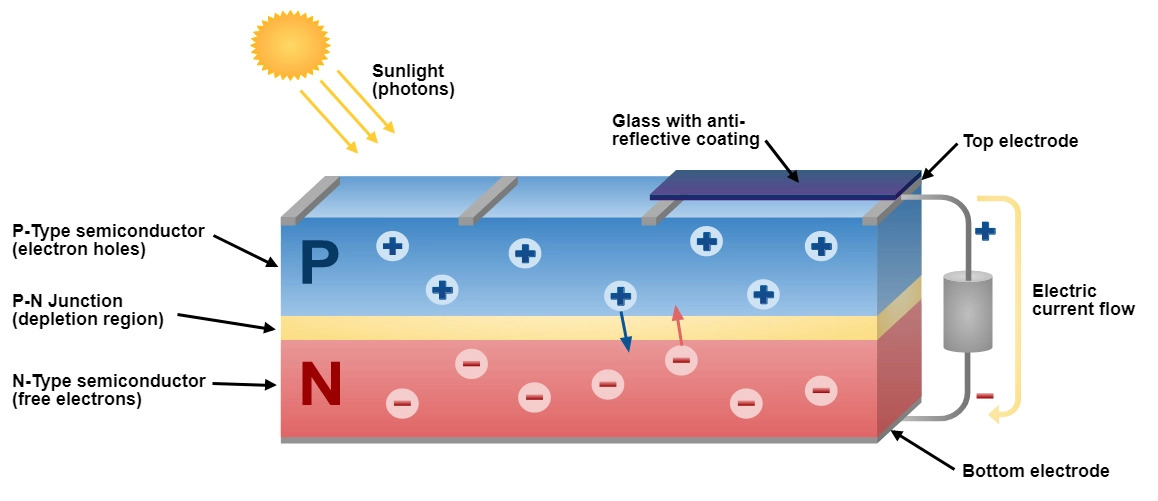
\includegraphics[width=1\textwidth]{Figures/photovoltaic_cell_diagram.jpg}
    \caption{An example figure.}
    \label{fig:photovoltaic_cell_diagram}
\end{figure}

\FloatBarrier

\noindent - In a photovoltaic cell, crystalline silicon is sandwiched between conductive layers.\par
\noindent - Each silicon atom is connected to its neighbours by four strong bonds.\par
\noindent - A silicon photovoltaic cell uses two different layers of silicon.\par
\begin{itemize}
    \item An n-type silicon, which has extra electrons.
    \item A p-type silicon has extra spaces for electrons, called holes.
\end{itemize}
\noindent - Where the two types of silicon meet, electrons can wander across the p/n junction, leaving a positive charge on one side and creating negative charge on the other.\par

\noindent - When a photon strikes the silicon cell with enough energy, it can knock an electron from it's bond, leaving a hole.\par
\noindent - The negatively charged electron and location of the positively charged hole are now free to move around.\par
\noindent - Because of the electric field at the p/n junction, they will only go one way.\par
\noindent - They electron is drawn to the n-side while the hole is drawn to the p-side.\par
\noindent - The mobile electrons are collected by thin metal fingers at the top of the cell.\par
\noindent - From there, they flow through an external circuit, doing electrical work, like powering a light bulb, before returning through the conductive aluminium sheet on the back.\par
\noindent - Each photovoltaic cell only puts out half a volt, but you can string them together in modules to get more power.\par
\noindent - Electrons are the only moving parts in a photovoltaic cell, and the go back to where they came from, so there is nothing to get worn out, or used up.\par
\noindent - Therefore, photovoltaic cells can last for decades.\vspace{0.5em}

\noindent \textit{So what is the reason that photovoltaic modules don't last forever -- Lead into the limitations of photovoltaic modules}






\subsection{Limitations of Photovoltaic Modules}
\begin{itemize}
    \item What are the limitations of photovoltaic modules?
\end{itemize}

\subsection{Heat Transfer in Photovoltaic Modules}
\begin{itemize}
    \item What is heat transfer?
    \item What are the types of heat transfer?
    \item What is the fundamental concept of heat transfer?
    \item What are some convection principles used to enhance heat transfer in a photovoltaic module?
\end{itemize}

\subsubsection{Vortex Induced Heat Transfer}
\begin{itemize}
    \item What is a vortex?
    \item How does a vortex/system of vortexes induce heat transfer?
    \item Are there any drawbacks of vortex-induced heat transfer? If so, what are they?
\end{itemize}

\subsubsection{Conduction}
\begin{itemize}
    \item What is conduction?
    \item How can conduction be used to enhance heat transfer?
    \item What are some examples of this principle in practice?
    \item What were the results of this practice?
    \item Are there any drawbacks of conduction as a method to enhance heat transfer?
\end{itemize}

\subsubsection{Radiation}
\begin{itemize}
    \item What is radiation?
    \item How can radiation be used to enhance heat transfer?
    \item What are some examples of this principle in practice?
    \item What were the results of this practice?
    \item Are there any drawbacks of radiation as a method to enhance heat transfer?
\end{itemize}

\subsection{Convective Photovoltaic Module Cooling Methods}
\begin{itemize}
    \item What is convection?
    \item What are some cooling methods for convective photovoltaic modules?
\end{itemize}

\subsubsection{Cooling through Natural Convection}
\begin{itemize}
    \item What is Natural Convection?
    \item How is natural convection used as a cooling method for photovoltaic modules?
    \item Are there drawbacks to natural convection as a cooling method for photovoltaic modules?
    \item How does forced convection compare to natural convection as a cooling method for photovoltaic modules?
\end{itemize}

\subsubsection{Cooling through Forced Convection}
\begin{itemize}
    \item What is forced convection?
    \item How is forced convection used as a cooling method for photovoltaic modules?
    \begin{itemize}
        \item DC Fan Experiment
        \item Floating Photovoltaic Module Experiment
    \end{itemize}
    \item Are there drawbacks to forced convection as a cooling method for photovoltaic modules?
    \item Air vs Water Cooling Experiment
    \item Air Cooled Modified Photovoltaic Module Experiment
    \item Single Fin vs Multiple Fin Experiment
\end{itemize}

\subsubsection{Cooling through Vortex Generators}
\begin{itemize}
    \item What is a vortex generator?
    \item What is the purpose of vortex generators?
    \item Examples of Vortex Generator Experiments in the Context of Photovoltaic Module Cooling
\end{itemize}